\documentclass[a4paper,11pt]{article}
		\usepackage[utf8]{inputenc}
	\usepackage[italian]{babel}
	\usepackage{hyperref}	%Consente l'inserimento di \url
	\usepackage{booktabs}	%Utilità di abbellimento tabelle
	\usepackage{longtable}
	\usepackage{tabularx}
	%\usepackage{widetable}
	\usepackage{array}
	\usepackage{listings}
	\usepackage{graphicx}
	\usepackage{caption}
	\usepackage{fancyhdr}
	\newenvironment{fixpic}{}{} % [1]
	\usepackage[a4paper,top=3cm,bottom=3cm,left=2.5cm,right=2.5cm]{geometry}
	%******
	\usepackage{makeidx}
	\usepackage{textcomp}
	\usepackage{multirow}
	\usepackage{rotfloat}
	\usepackage{lastpage}
	\usepackage{array}
	\usepackage{float}
	% *************************************
	% QUI CODICE PER \SUBSUBSUBSECTION
	\usepackage{titlesec}
	\titleclass{\subsubsubsection}{straight}[\subsection]
	
	\newcounter{subsubsubsection}[subsubsection]
	\renewcommand\thesubsubsubsection{\thesubsubsection.\arabic{subsubsubsection}}
	\renewcommand\theparagraph{\thesubsubsubsection.\arabic{paragraph}} % optional; useful if paragraphs are to be numbered
	
	\titleformat{\subsubsubsection}
	  {\normalfont\normalsize\bfseries}{\thesubsubsubsection}{1em}{}
	\titlespacing*{\subsubsubsection}
	{0pt}{3.25ex plus 1ex minus .2ex}{1.5ex plus .2ex}
	
	\makeatletter
	\renewcommand\paragraph{\@startsection{paragraph}{5}{\z@}%
	  {3.25ex \@plus1ex \@minus.2ex}%
	  {-1em}%
	  {\normalfont\normalsize\bfseries}}
	\renewcommand\subparagraph{\@startsection{subparagraph}{6}{\parindent}%
	  {3.25ex \@plus1ex \@minus .2ex}%
	  {-1em}%
	  {\normalfont\normalsize\bfseries}}
	\def\toclevel@subsubsubsection{4}
	\def\toclevel@paragraph{5}
	\def\toclevel@paragraph{6}
	\def\l@subsubsubsection{\@dottedtocline{4}{7em}{4em}}
	\def\l@paragraph{\@dottedtocline{5}{10em}{5em}}
	\def\l@subparagraph{\@dottedtocline{6}{14em}{6em}}
	\makeatother
	
	\setcounter{secnumdepth}{4}
	\setcounter{tocdepth}{4}
	%FINE \SUBSUBSUBSECTION
	%****************************************
	%STYLE PER INSERIMENTO DEL CODICE
	\lstdefinestyle{style1}{
	  belowcaptionskip=1\baselineskip,
	  breaklines=true,
	  frame=L,
	  xleftmargin=\parindent,
	  language=Pascal,
	  showstringspaces=false,
	  basicstyle=\footnotesize\ttfamily,
	  keywordstyle=\bfseries\color{blue},
	  commentstyle=\itshape\color{blue},
	  identifierstyle=\color{blue},
	  stringstyle=\color{orange},
	}
	
	\lstdefinestyle{style2}{
	  belowcaptionskip=1\baselineskip,
	  frame=L,
	  xleftmargin=\parindent,
	  language=C,
	  basicstyle=\footnotesize\ttfamily,
	  commentstyle=\itshape\color{blue},
	}
	\lstset{style=style1}
	
	%FINE STYLE INSERIMENTO CODICE
	%*****************************************
	\usepackage[default]{cantarell} %% Use option "defaultsans" to use cantarell as sans serif only
	\usepackage[T1]{fontenc}        %% for font
	\hypersetup{colorlinks, linkcolor=black, urlcolor=blue}
	\newcommand{\addglos}{\begin{scriptsize}{\textbf{\ped{G}}} \end{scriptsize}} 
	\pagestyle{fancy}
	\fancyhead{}
	\fancyfoot{}
	%\fancyhead[L]{
\includegraphics[scale=0.28]{team_not_found.jpeg}}
	\fancyhead[L]{
\includegraphics[scale=0.15]{../../team404_small.jpg} \hspace{2mm} QUIZZIPEDIA}
	\fancyhead[R]{\leftmark}
	\fancyfoot[L]{Universit\`a degli studi di Padova - IS 2015/2016 \\ \url{team404swe@gmail.com}}

	
	%Commando usato per la tabella di informazioni sul documento
	\newcommand{\introtab}[9]{
		\begin{table}[ht]
		\begin{center}		
		\begin{tabular}{r l}			
			\toprule		
			\multicolumn{2}{c}{\textbf{ Informazioni sul documento }} \\
			\midrule 
			\textbf{Nome Documento}			& \vline \hspace{3.5 mm} {#1} \\
			\textbf{Versione}				& \vline \hspace{3.5 mm} {#2} \\
			\textbf{Uso} 					& \vline \hspace{3.5 mm} {#3} \\
			\textbf{Data Creazione} 		& \vline \hspace{3.5 mm} {#4} \\
			\textbf{Data Ultima Modifica} 	& \vline \hspace{3.5 mm} {#5} \\
			\textbf{Redazione}				& \vline \hspace{3.5 mm} {#6} \\
											%& \vline \hspace{3.5 mm} {#7} \\	
			\textbf{Verifica} 				& \vline \hspace{3.5 mm} {#7}	\\
			\textbf{Approvazione}			& \vline \hspace{3.5 mm} {#8}\\	
			\textbf{Committente} 			& \vline \hspace{3.5 mm} Zucchetti SPA\\
			\textbf{Lista di distribuzione} & \vline \hspace{3.5 mm} Prof. Vardanega Tullio \\														& \vline \hspace{3.5 mm} TEAM404 \\
	\bottomrule	
	\end{tabular}
	\end{center}
	\end{table}
	}
	% Comando di inizio del registro
	\newcommand{\beginregistro}{
		%\begin{longtable}{{|p{0.10\textwidth}|p{0.20\textwidth}|p{0.15\textwidth}|p{0.50\textwidth}|}}
		\begin{longtable}{{|p{1.5cm}|p{2.5cm}|p{2cm}|p{8cm}|}} 
	 		\hline	
	}
	% commando usato pr inserire una riga al registro delle modifiche
	\newcommand{\rigaregistro}[4]{
		{\footnotesize #1} & {\footnotesize #2} &  {\footnotesize #3} &  {\footnotesize #4} \\
			\hline	
	}
	% Comando di fine registro
	\newcommand{\fineregistro}{ \end{longtable}	}
	
	%************************************************
	% commandi per il GLOSSARIO
	%***********************************************
	% Commando di inizio tabella Glossario
	\newcommand{\beginglos}{
		\begin{longtable}{{p{0.20\textwidth}p{0.65\textwidth}}}	
	}
	% Commando per i termini del glossario
	
	\newcommand{\itemglos}[2]{
		\textbf{#1 :} & {#2} \\ \\ \\
	}
	% Commando fine Glossario
	\newcommand{\fineglos}{ \end{longtable} }
	% Comando per aggiungere una ssezione numerata con lettere al glossario
	\newcommand{\sezione}{
	\subsection{}	
	\rule[0.3pt]{\linewidth}{0.4pt} \\ % Linea orizzontale
	}
	
\newcommand{\sezioneglos}[1] { 
  \newpage
  \cleardoublepage
  \phantomsection
  \addcontentsline{toc}{section}{#1}
  \vspace{11pt}
  \textbf{\huge{#1} } % Lettera grande 
  \\
  \rule[0.3pt]{\linewidth}{0.4pt} \\ % Linea orizzontale
  \fancyhead[R]{#1}
}
	\newcommand{\code}[1]{\texttt{#1}}

	\title{\textbf{{\fontsize{8mm}{5mm}\selectfont QUIZZIPEDIA}}}
	\date{}
	\author{}	


\begin{document}
	\maketitle
	\thispagestyle{empty}
	\begin{center}	
	
\includegraphics{../team_not_found.jpg}\\
	\fontsize{5mm}{3mm}\url{team404swe@gmail.com}\\
	
	\vspace{50mm}
	\textbf{Manuale Utente 1.0}
	\end{center}
	\introtab{Manuale Utente}	%1 nome documento
			{2.0} 							%2 versione
			{Esterno} 						%3 Uso
			{16 agosto 2016} 				%4 Data cre
			{\today} 						%5 Data mod
			{Luca Alessio}		%6 Redazione
			{Martin V. Mbouenda} 			%7 Verifica
			{Davide Bortot} 				%8 Approvazione
	\newpage
	\thispagestyle{empty}
	\null  

	\newpage
	\newpage
	\fancyhead[R]{REGISTRO DELLE MODIFICHE}
	\fancyfoot[R]{\thepage}
	
	\hspace{30 mm}
	\section*{Registro delle modifiche}
	
	\beginregistro
	
	\rigaregistro{\textbf{Versione}}{\textbf{Autore}}{\textbf{Data}}		 {\hspace{5 mm}}
	\rigaregistro{1.0.0}{Davide Bortot (Responsabile)}{22/06/2016}{Approvazione documento}
	\rigaregistro{0.0.16}{Luca Alessio (Verificatore)}{22/06/2016}{Verifica documento}
	\rigaregistro{0.0.15}{Luca Alessio (Verificatore)}{21/06/2016}{Stesura sezione "Sintassi QML"}
	\rigaregistro{0.0.14}{Luca Alessio (Verificatore)}{20/06/2016}{Stesura sezione "Creazione Questionario"}
	\rigaregistro{0.0.13}{Davide Bortot (Responsabile)}{20/06/2016}{Caricamento immagini}
	\rigaregistro{0.0.12}{Andrea Multineddu (Programmatore)}{20/06/2016}{Stesura sezione "Installazione"}
\rigaregistro{0.0.11}{Luca Alessio (Verificatore)}{19/06/2016}{Stesura sezione "Creazione Domanda"}
\rigaregistro{0.0.10}{Luca Alessio (Verificatore)}{19/06/2016}{Stesura sezione "Profilo Utente"}
\rigaregistro{0.0.9}{Luca Alessio (Verificatore)}{19/06/2016}{Stesura sezione "Svolgimento di un Questionario"}
\rigaregistro{0.0.8}{Luca Alessio (Verificatore)}{19/06/2016}{Stesura sezione "Scelta di un Questionario"}	
	\rigaregistro{0.0.7}{Luca Alessio (Verificatore)}{18/06/2016}{Stesura sezione "Scelta di un questionario"}
	\rigaregistro{0.0.6}{Luca Alessio (Verificatore)}{18/06/2016}{Stesura sezioni "Registrazione" e "Autenticazione"}
	\rigaregistro{0.0.5}{Luca Alessio (Verificatore)}{18/06/2016}{Stesura sezione "L'applicazione a prima vista"}
	\rigaregistro{0.0.4}{Andrea Multineddu (Programmatore)}{17/06/2016}{Inserimento immagini}
	\rigaregistro{0.0.3}{Luca Alessio (Verificatore)}{16/06/2016}{Stesurea sezione "Requisiti di sistema"}
	\rigaregistro{0.0.2}{Luca Alessio (Verificatore)}{16/06/2016}{Stesura sezione "Introduzione"}
	\rigaregistro{0.0.1}{Luca Alessio (Verificatore)}{16/06/2016}{Creazione del documento}
	
	\fineregistro

	\newpage
	\fancyhead[R]{\leftmark}
	\tableofcontents
	\pagenumbering{Roman}
	\newpage
	\listoffigures
	\listoftables
	
	\newpage
	\pagenumbering{arabic}
	
	\section*{Sommario}
	Questo documento rappresenta il Manuale Utente per il software Quizzipedia sviluppato dal Team404 per conto di Zucchetti S.p.A. ed ha lo scopo di illustrare all'utente le modalità di utilizzo e i servizi offerti dell'applicazione.
	
	\newpage
	\section{Introduzione}
	\subsection{Scopo del documento}
	Il documento ha lo scopo di definire nel dettaglio la struttura del sistema Quizzipedia, approfondendone la descrizione già definita nel documento di Specifica Tecnica. Per ogni package del sistema verrà data una descrizione estensiva delle sue classi. Per poter sviluppare al meglio il prodotto, i programmatori dovranno attenersi alle specifiche definite in questo documento.
	
	\subsection{Scopo del prodotto}
	Il progetto \textbf{Quizzipedia} ha come obiettivo lo sviluppo di un sistema software basato su tecnologie Web (Javascript\addglos, Node.js\addglos, HTML5\addglos, CSS3\addglos) che permetta la creazione, gestione e fruizione di questionari. Il sistema dovrà quindi poter archiviare i questionari suddivisi per argomento, le cui domande dovranno essere raccolte attraverso uno specifico linguaggio di markup (Quiz Markup Language) d'ora in poi denominato QML\addglos. In un caso d'uso a titolo esemplificativo, un "esaminatore" dovrà poter costruire il proprio questionario scegliendo tra le domande archiviate, ed il questionario così composto sarà presentato e fruibile all' "esaminando", traducendo l'oggetto QML in una pagina HTML\addglos, tramite un'apposita interfaccia web. Il sistema presentato dovrà inoltre poter proporre questionari preconfezionati e valutare le risposte fornite dall'utente finale.
	\\
	Per un'analisi più precisa ed approfondita del progetto si rimanda al documento\\ "\textit{analisi\_dei\_requisiti\_4.0.pdf}".
	\subsection{Glossario}
	Viene allegato un glossario nel file ``\textit{glossario\_4.0.pdf}'' nel quale viene data una definizione a tutti i termini che in questo documento appaiono con il simbolo '\addglos' a pedice.
	\subsection{Riferimenti}
		\subsubsection{Normativi}

		\begin{itemize}
			\item Capitolato d'appalto Quizzipedia:\\
			\url{http://www.math.unipd.it/~tullio/IS-1/2015/Progetto/C5.pdf}
			\item Norme di Progetto: "\textit{norme\_di\_progetto\_4.0.pdf}"
		\end{itemize}
		\subsubsection{Informativi}
		\begin{itemize}
			\item Corso di Ingegneria del Software anno 2015/2016:\\
			\url{http://www.math.unipd.it/~tullio/IS-1/2015/}
			\item Regole del progetto didattico:\\
			\url{http://www.math.unipd.it/~tullio/IS-1/2015/Dispense/PD01.pdf}\\
			\url{http://www.math.unipd.it/~tullio/IS-1/2015/Progetto/}
			\item Specifica Tecnica: "\textit{specifica\_tecnica\_3.0.pdf}"
			\item Framework Meteor:\\
			\url{https://www.meteor.com/}
			\item Framework AngularJs:\\
			\url{https://www.angularjs.org/}
		\end{itemize}
	\pagebreak
	\newpage
\section{Requisiti di Sistema}
Quizzipedia è un'applicazione web, pertanto è mandatorio che il dispositivo utilizzato sia connesso ad internet. Per quanto riguarda l'hardware del dispositivo, non sono invece richieste particolari specifiche.
\subsection{Browser supportati}
Quizzipedia supporta i seguenti browser:
\begin{itemize}
	\item Chrome
	\item Firefox 7+
	\item Internet Explorer 8+
	\item Safari 4+
	\item Android stock web browser
	\item IOS stock web browser
	\item Opera Desktop e Mobile
\end{itemize}

\section{Installazione}
In ambiente Windows l'utente deve installare Meteor per poter usufruire dell'applicazione.
Meteor e' scaricabile tramite il sito ufficiale del framework Meteor \url{https://www.meteor.com/install}.\\
Dopo aver completato il download del pacchetto di installazione, l'utente deve avviarlo e completare l'installazione dello stesso. \\ \\In ambiente MAC e Linux l'utente deve installare il framework Meteor eseguendo da terminale il comando: \\ \code{curl https://install.meteor.com/ | sh}\\
e portare a completamento la procedura di installazione.\\ \\Per poter utilizzare il progetto (indipendentemente dall'ambiente di lavoro) è necessario spostarsi nella
cartella del progetto meteor ed eseguire il comando \code{meteor} tramite terminale o prompt dei comandi.\\
Meteor preparera' il nostro progetto per essere utilizzabile tramite browser e appena verra' stampata sul terminale la riga: \code{App running at: http://localhost:3000/}
sara' possibile utilizzare la nostra applicazione tramite qualsiasi browser moderno collegandosi all'indirizzo \url{localhost:3000}.
	\newpage
	\section{L'applicazione a prima vista}
	All'accesso dell'utente l'applicazione si presenta come segue:\\
	\begin{figure}[h!]
	\begin{center}
	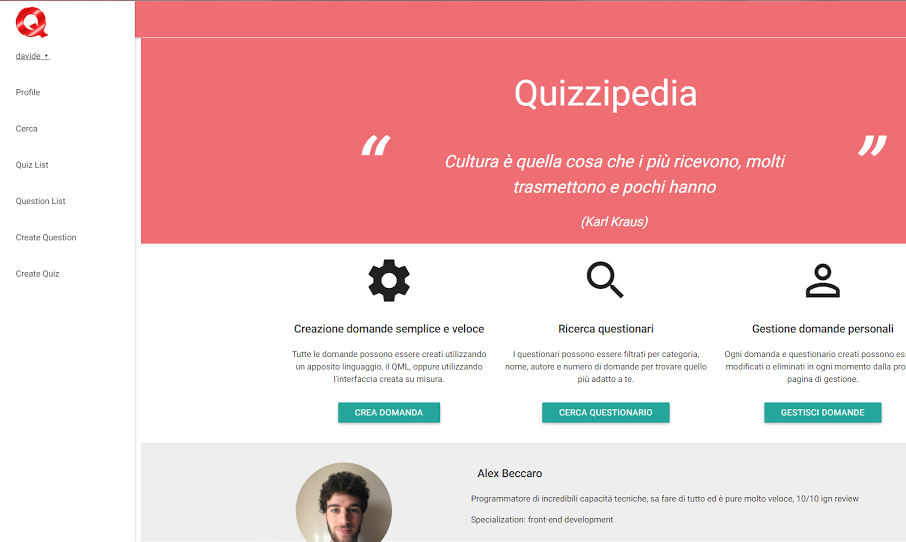
\includegraphics[scale=0.5]{../images/screen_home.png}
	\caption{Home Page}
	\end{center}
	\end{figure}\\
	L'utente ha la possibilità partire direttamente con la risoluzione di un questionario o di autenticarsi nel sistema per usufruire delle funzionalità di gestione di domande e questionari che vedremo nel dettaglio nei seguenti paragrafi.\\ \\
	Per la home page si è scelto di adottare un layout il più possibile minimale per renderlo semplice e accessibile ad ogni tipologia di utenza.\\
	Da ogni pagina del sito è possibile usufruire del comodo menù di navigazione laterale che elenca le funzionalità disponibili del sistema (alcune come ad esempio la creazione della domanda potrebbero essere bloccate qualora l'utente non abbia ancora effettuato l'accesso).
	\newpage
	\section{Registrazione}
	Per poter usufruire delle funzionalità più avanzate di Quizzipedia, l'utente deve necessariamente creare il proprio account nel sistema.\\
	L'utente può trovare il modulo di registrazione in alto a sinistra alla voce "Register", il modulo si presenta come segue:\\
	\begin{figure}[h!]
	\begin{center}
	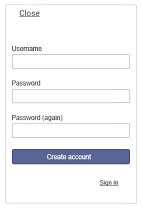
\includegraphics[scale=0.85]{../images/form.png}
	\caption{Form di registrazione}
	\end{center}
	\end{figure}	
	\\
	E' necessario inserire nei corrispondenti campi un indirizzo email valido e una password che va ripetuta per evitare errori di battitura.\\ \\
	Se i dati inseriti sono corretti, alla pressione del tasto "Create Account" il nuovo profilo dell'utente verrà effettivamente creato e l'utente potrà accedere a tutte le funzionalità di Quizzipedia, in caso contrario verrà notificato da un messaggio d'errore appropriato.
	\section{Autenticazione}
	L'autenticazione nel sistema segue lo stesso principio della registrazione: si accede al form dalla voce nel menù Sign In, si inseriscono le proprie credenziali e si logga così nel sistema.\\ Se i dati inseriti non sono corretti ancora una volta l'utente viene notificato da un messaggio d'errore. 
	\newpage
	\section{Scelta di un Questionario}
	La scelta del questionario si svolge su due livelli, prima avviene la scelta della categoria e poi avviene la scelta del singolo questionario presente tra i vari possibili questionari della stessa categoria.
	\begin{figure}[h!]
	\begin{center}
	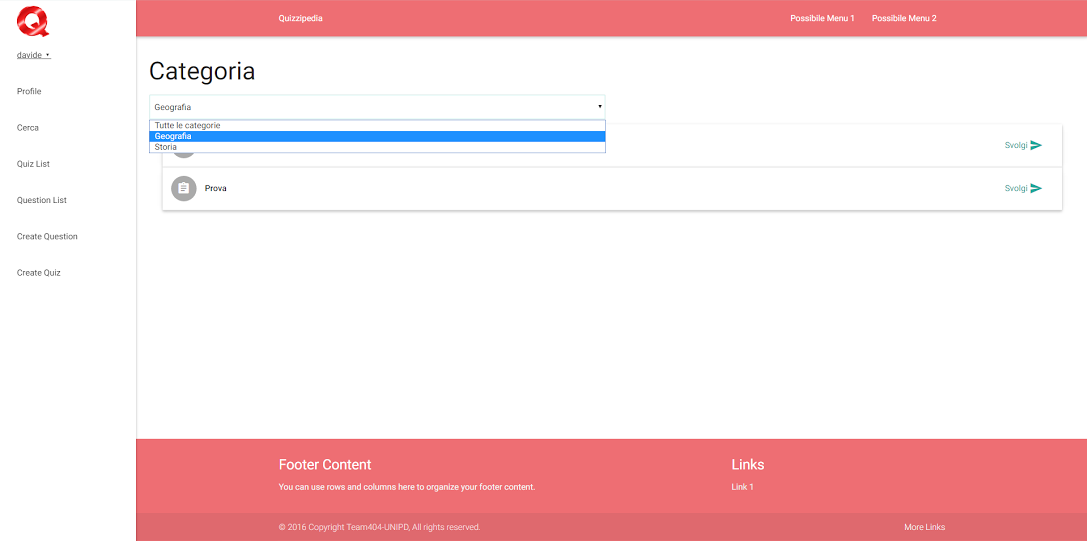
\includegraphics[scale=0.5]{../images/screen_category.png}
	\caption{Menù selezione categoria questionario}
	\end{center}
	\end{figure}
	\\
	Ad ogni questionario è abbinata una breve descrizione generale sugli argomenti che tratta.\\ E' possibile cominciare un questionario semplicemente cliccando sul tasto Svolgi.
	\newpage
	\section{Svolgimento di un Questionario}
	Durante l'esecuzione di un questionario  all'utente si presenta la seguente interfaccia:\\
	\begin{figure}[h!]
	\begin{center}
	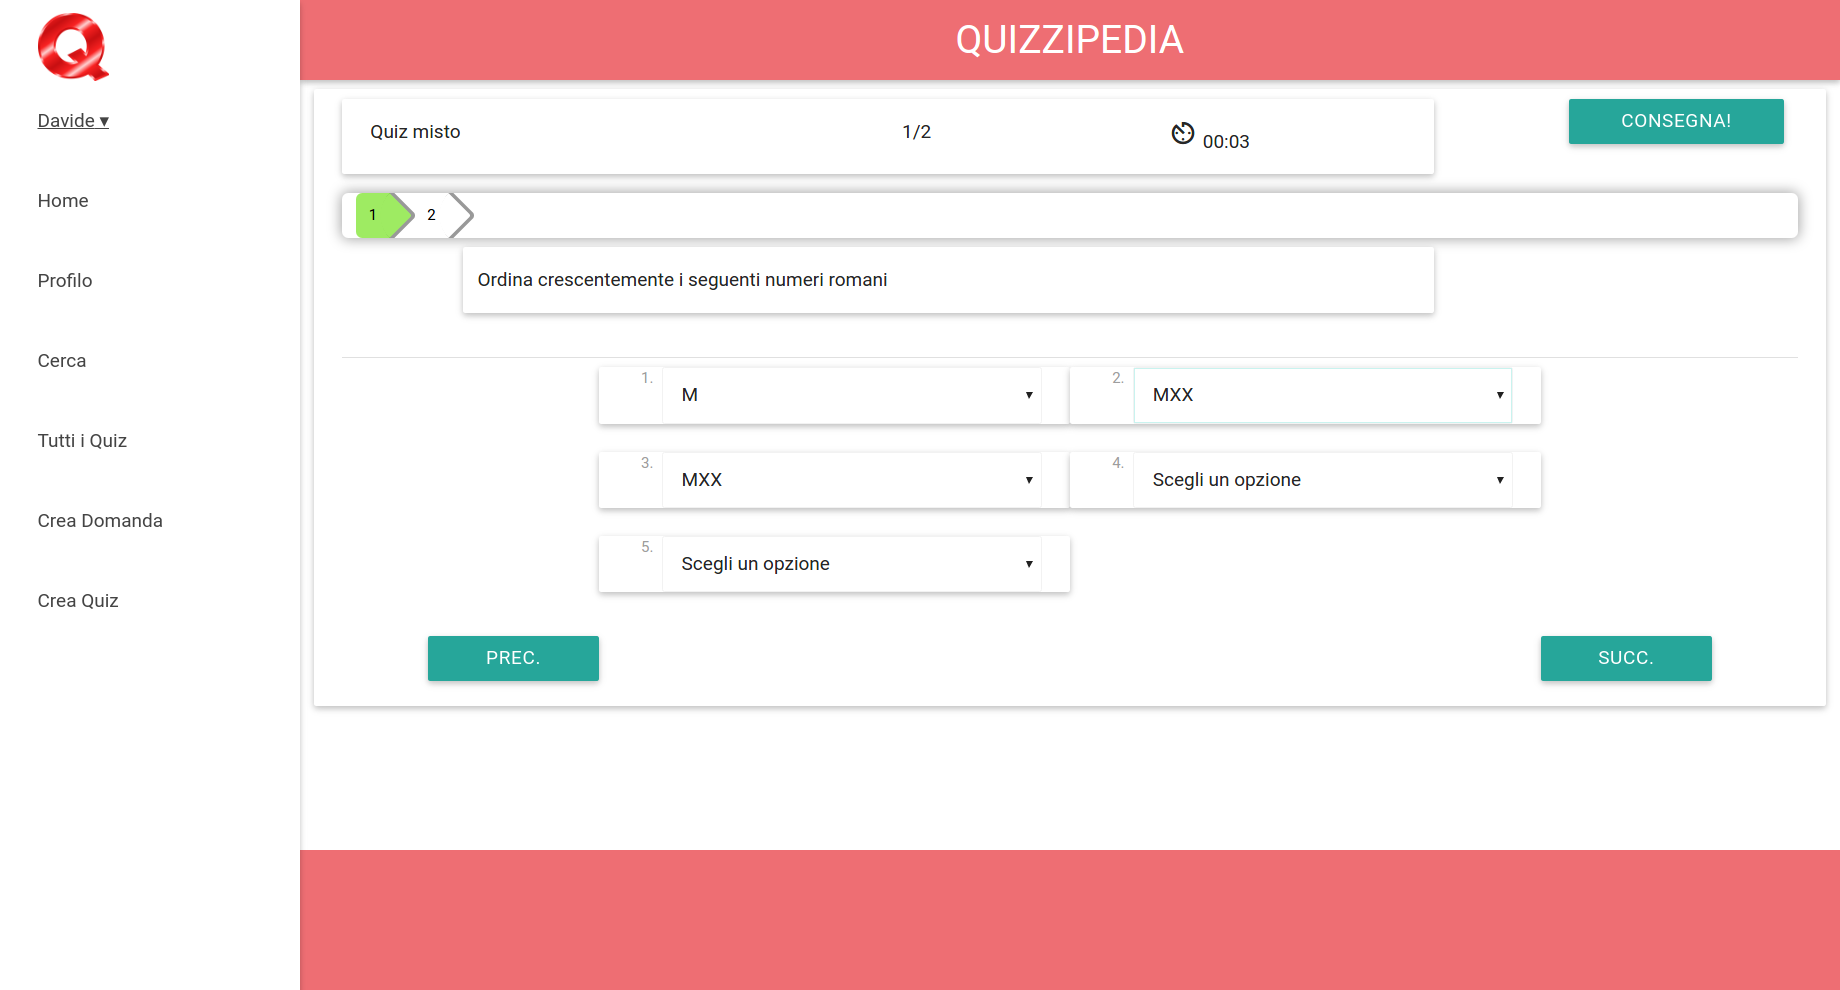
\includegraphics[scale=0.3]{../images/quizCompilation1.png}
	\caption{Esempio di domanda a ordinamento}
	\end{center}
	\end{figure}
	\\
	
	Dall'alto verso il basso da sinistra verso destra sono presenti rispettivamente:
	\begin{itemize}
	\item nome del questionario
	\item numero di domande completate
	\item tempo rimanente
	\item pulsante Consegna per la terminazione del questionario
	\item testo della domanda
	\item risposte della domanda (la struttura varia in base alla tipologia)
	\item tasto Precedente per tornare alla domanda precedente
	\item tasto Successivo per visitare la domanda successiva
	\end{itemize}
	
%	\begin{figure}[h!]
%	\begin{center}
%	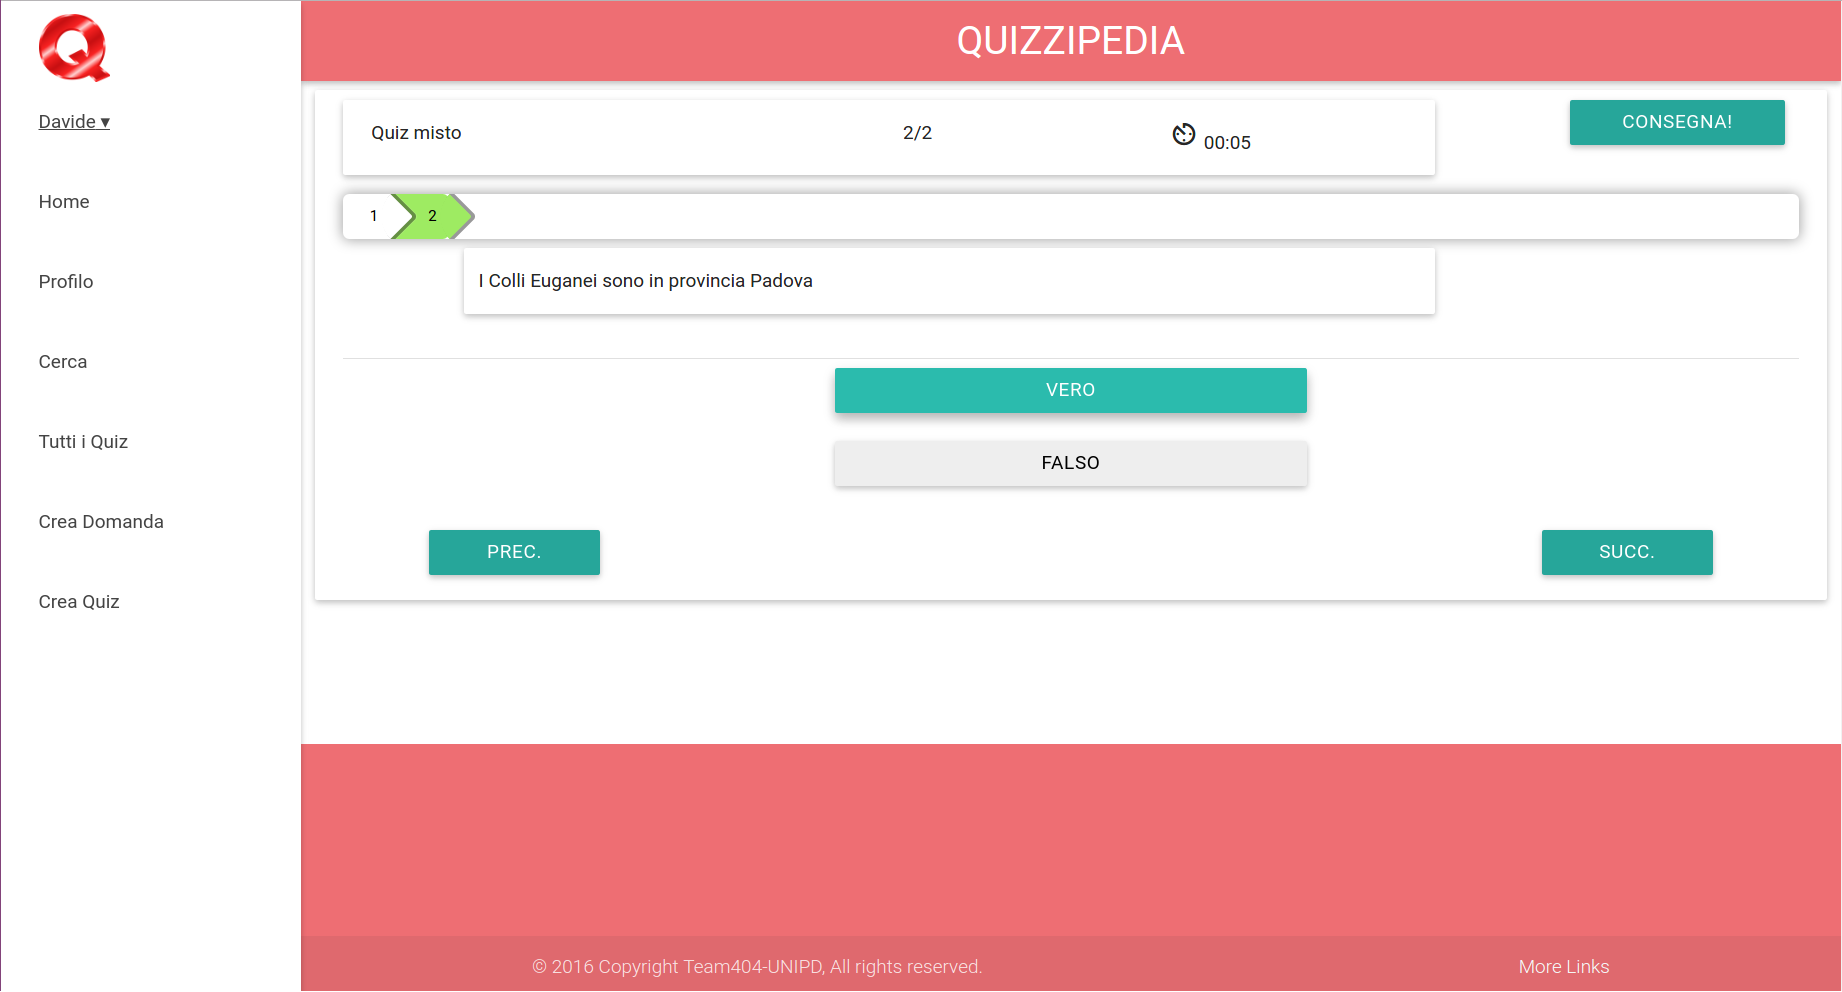
\includegraphics[scale=0.3]{../images/quizCompilation2.png}
%	\caption{Esempio di domanda vero o falso}
%	\end{center}
%	\end{figure}
%	\\
	\newpage
	\section{Profilo Utente}
	Il profilo utente è accessibile una volta autenticati dalla voce in alto a sinistra contenente il proprio nome utente.\\
	\begin{figure}[h!]
	\begin{center}
	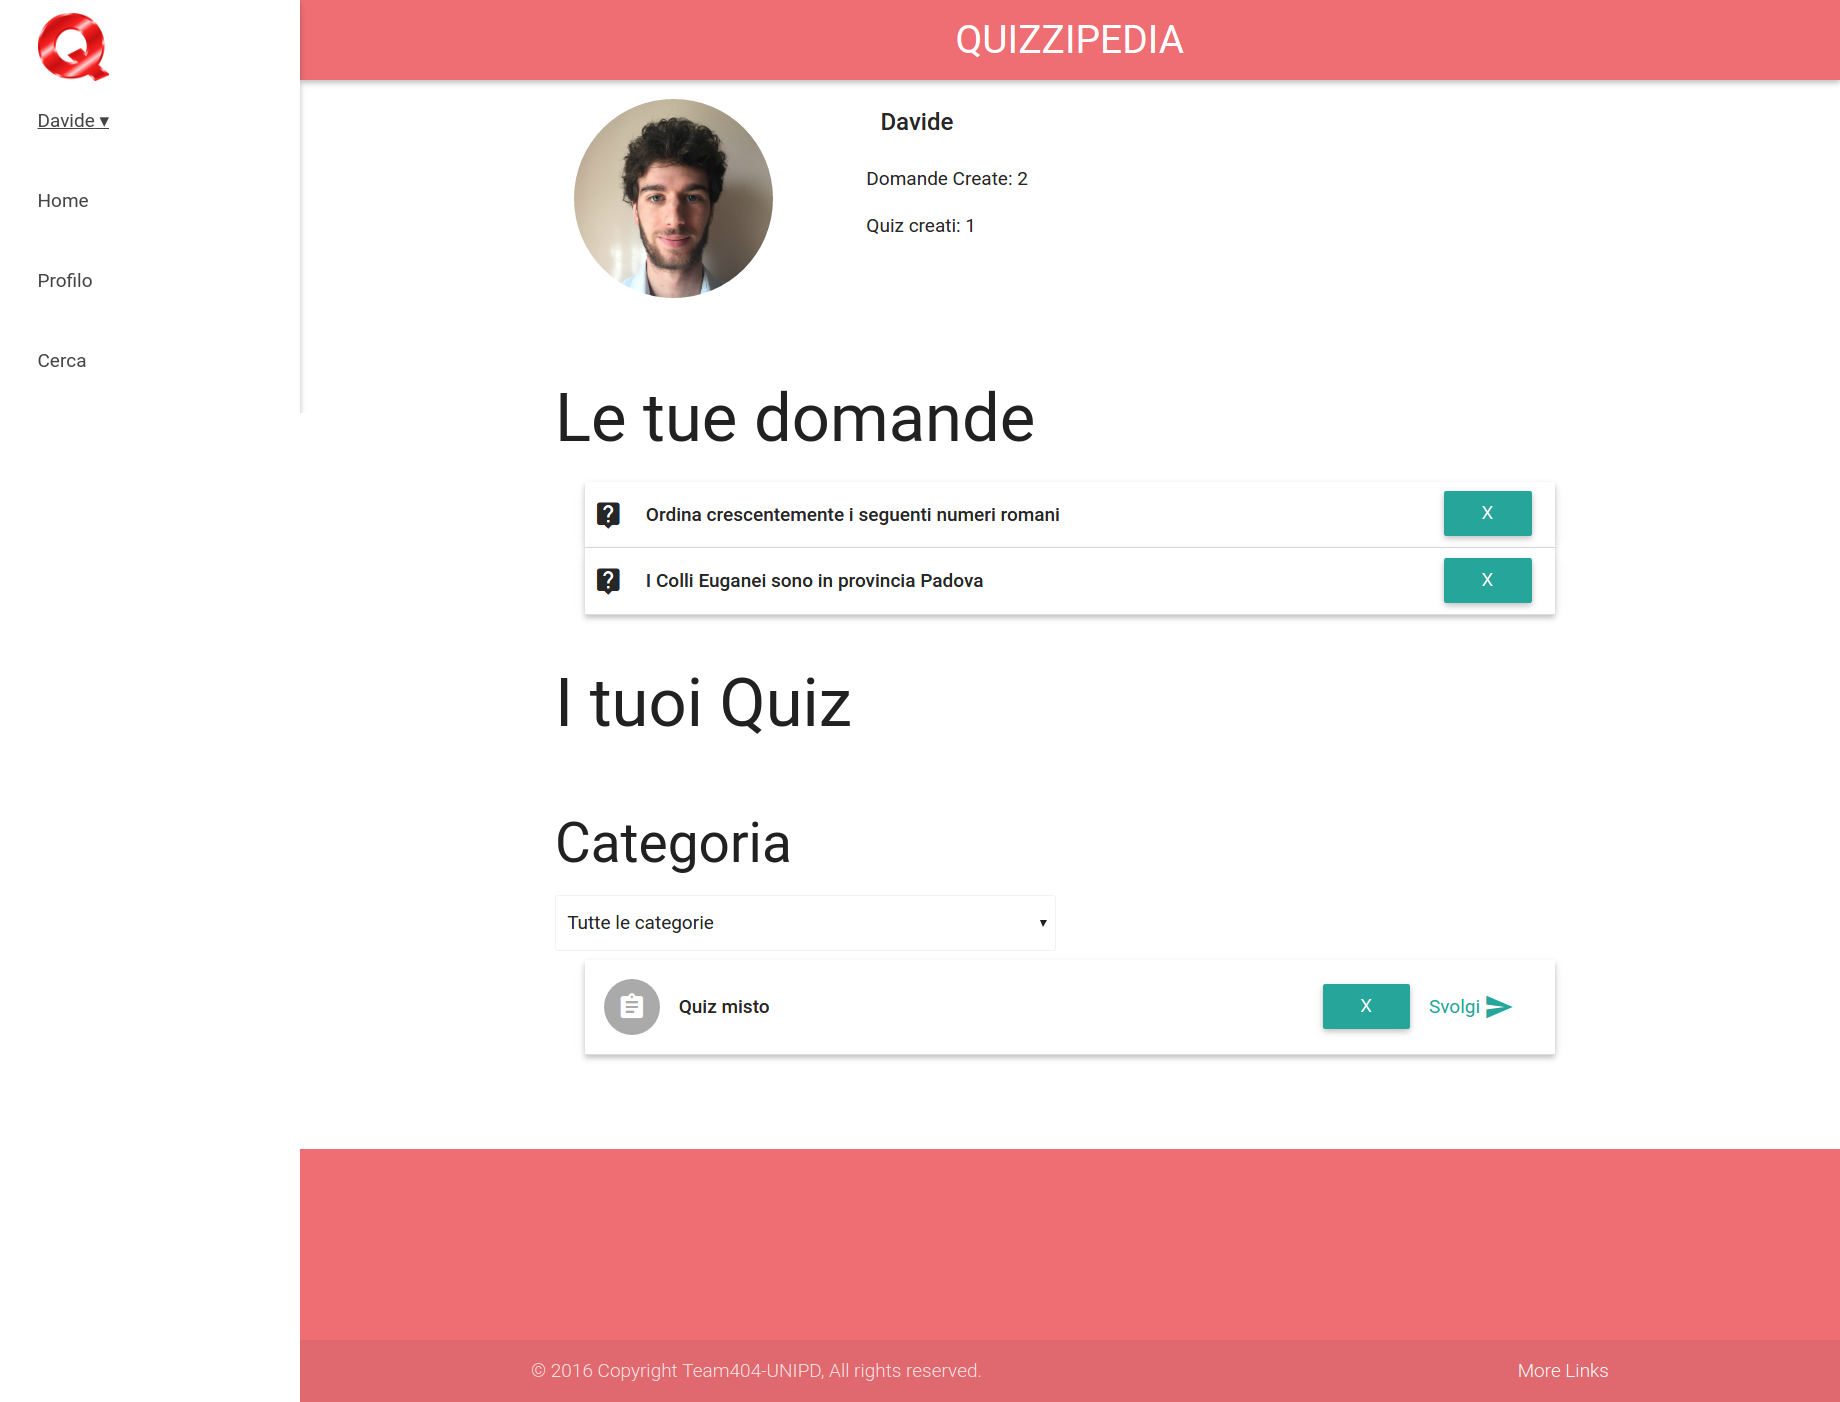
\includegraphics[scale=0.3]{../images/screen_profile.png}
	\caption{Profilo Utente}
	\end{center}
	\end{figure}
	\\
	Dal proprio profilo l'utente ha la possibilità di visualizzare le domande e i questionari creati finora.
	E' possibile eliminare singole domande o questionari cliccando sul pulsante X affiancato.\\ 
	\newpage
	\section{Creazione Domanda}
	E' possibile creare una domanda in due modi interagendo con il seguente form dove semplicemente andrà inserita la corretta sintassi QML della domanda (vedi sezione apposita del presente manuale).\\
	
	\begin{figure}[h!]
	\begin{center}
	\includegraphics[scale=0.2]{../images/QuestionFormQML.png}
	\caption{Creazione Domanda}
	\end{center}
	\end{figure}
	
	\newpage
	\section{Creazione Questionario}
	E' possibile creare un questionario nell'apposita sezione dell'applicazione accessibile solo ad utenti autenticati.\\
	\begin{figure}[h!]
	\begin{center}
	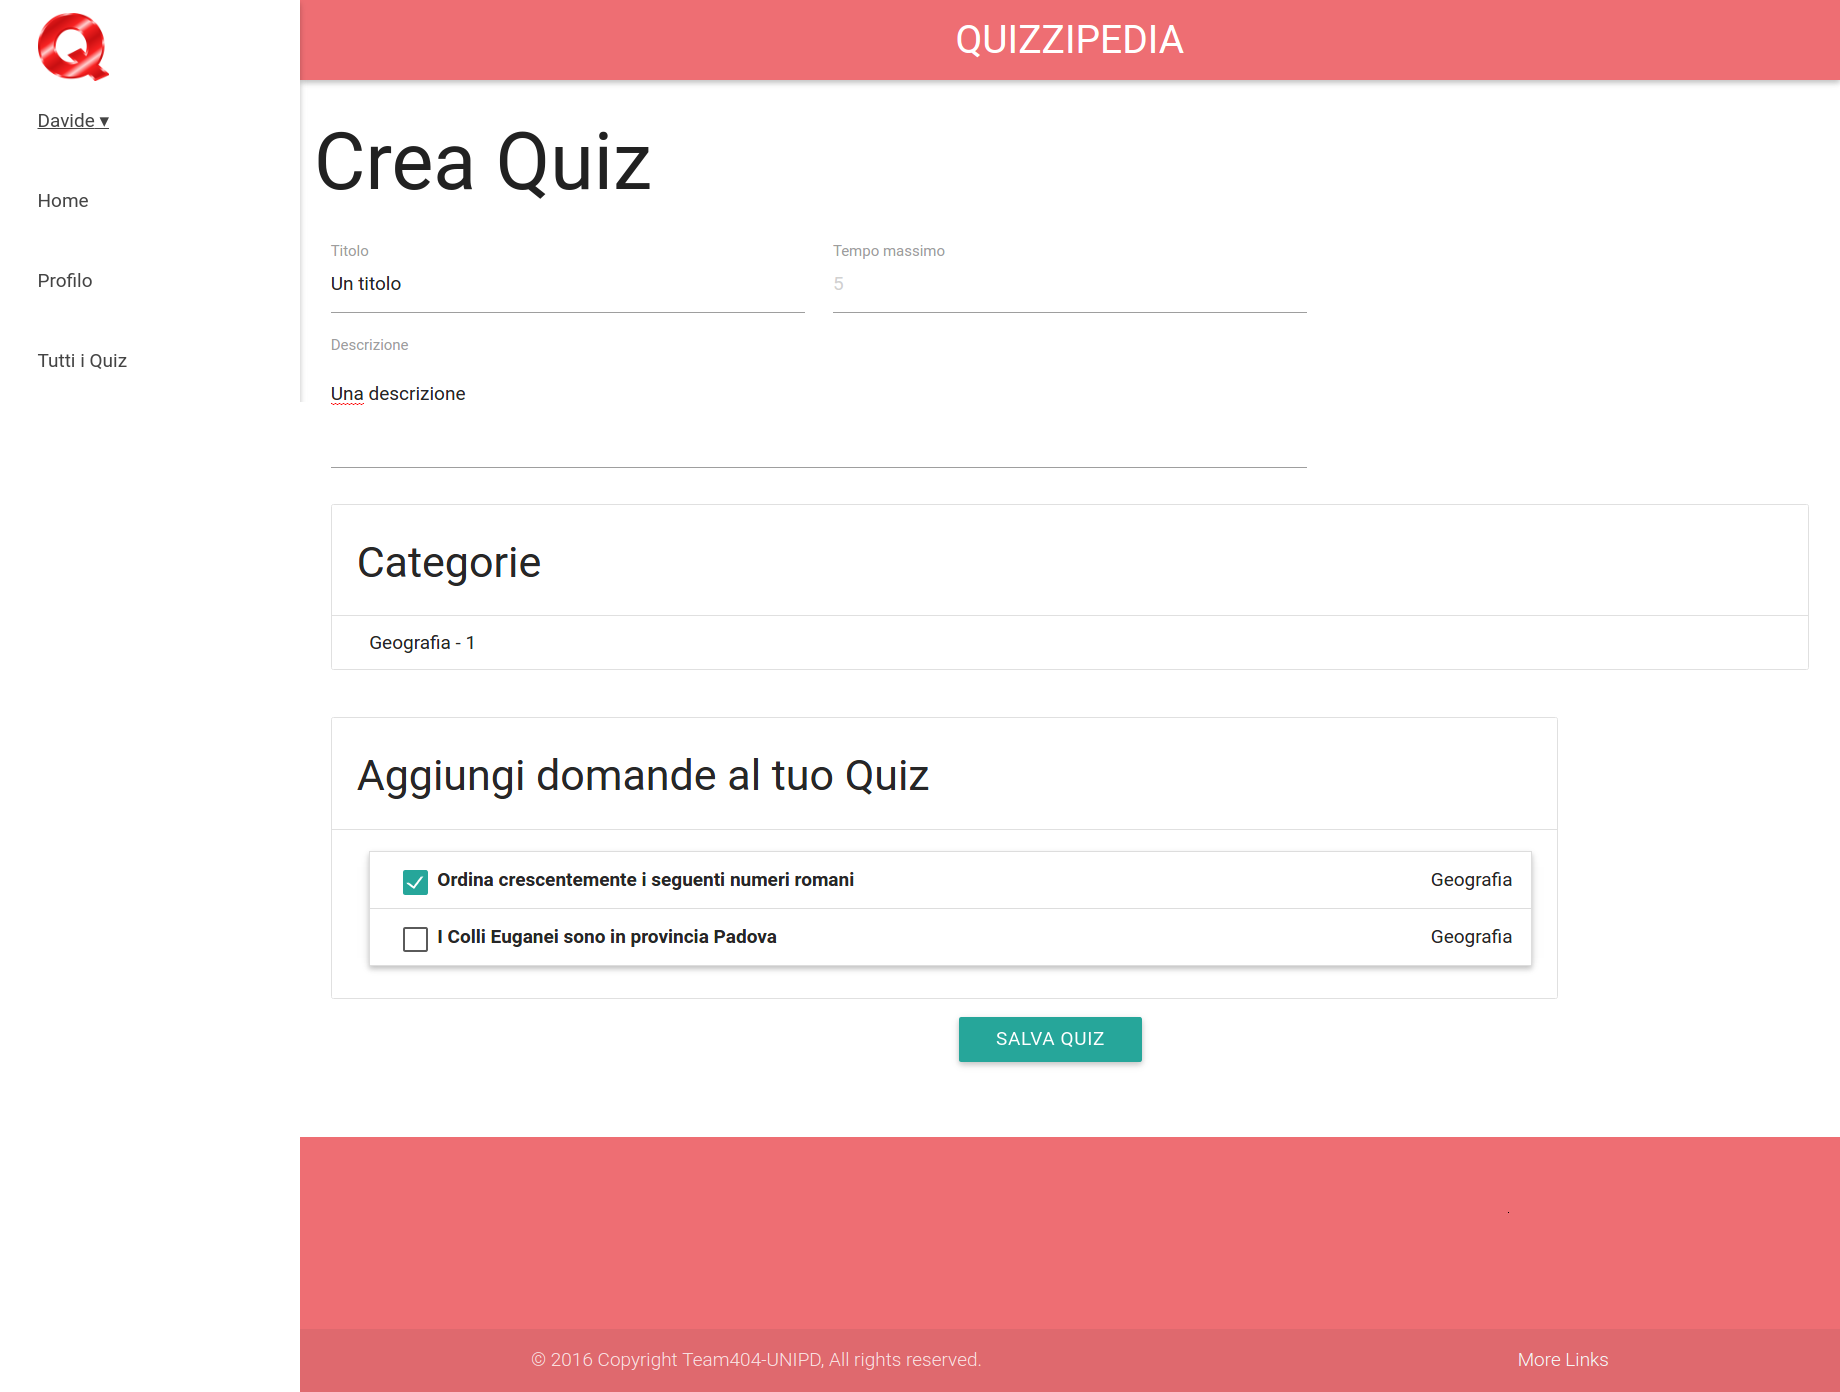
\includegraphics[scale=0.3]{../images/quizCreationForm.png}
	\caption{Creazione Questionario}
	\end{center}
	\end{figure}
	\\
	Durante la creazione vengono richiesti un titolo, una categoria e un tempo massimo.\\ L'utente può poi proseguire con la scelta delle domande da inserire nel questionario appartenenti alla categoria scelta tra quelle già presenti nel sistema (create in precedenza dall'utente stesso o da altri utenti).\\ Una volta completata la scelta delle domande da inserire è sufficente cliccare su Salva Quiz ed il quiz sarà così disponibile alla risoluzione per tutti gli utenti di Quizzipedia.
	\newpage
	\section{Sintassi QML}
	Le domande contenute nell'applicazione sono strutturate seguendo la sintassi \textit{Question Markup Language} creata appositamente dal Team404, questa sintassi si basa su delle espressioni regolari utilizzate da un parser e da un interpreter interni per assicurare la correttezza dei dati inseriti e per convertirli nel formato richiesto. \\ In questo manuale non affronteremo tuttavia il funzionamento di QML nel dettaglio in quanto ciò esula dagli scopi del presente documento.\\	
Una domanda QML è formata dai seguenti elementi:
\begin{itemize}
\item tipo della domanda
\item testo della domanda
\item elenco delle risposte
\item (opzionale) immagine allegata
\end{itemize}
Possiamo riscontrare la loro presenza in un questo esempio di domanda a risposta multipla:\\
\code{
<question type =" MU">\\
	<text>Quanto è alto il Monte Bianco?</text>\\
	<answer isRight =" yes"> 4809 m </answer >\\
	<answer isRight =" no"> 3540 m </answer >\\
	<answer isRight =" no"> 5011 m </answer >\\
</ question >\\}


Analizziamo uno per uno gli elementi.
\subsection{Tipologia Domanda}
Ogni domanda è racchiusa nel tag \code{<question>} che contiene anche l'attributo \code{type}.\\
Il valore di questo attributo cambia in base alla tipologia di domanda che si intende creare:
\begin{itemize}
\item \textbf{VF}: domanda di tipo vero/falso
\item \textbf{MU}: domanda a risposta a scelta multipla con una sola risposta giusta
\item \textbf{MX}: domanda a risposta a scelta multipla con più risposte giuste
\item \textbf{AS}: domanda di associazioni tra elementi dell'insieme A ed elementi dell'insieme B
\item \textbf{OD}: domanda di ordinamento delle risposte date
\end{itemize}
Nel caso si volesse allegare un'immagine alla domanda si deve aggiungere l'attributo \textbf{image} a cui va assegnato il percorso relativo dell'immagine da allegare.\\
\newpage
\subsection{Corpo della domanda}
All'interno del tag \code{<text>} va inserito solamente il testo formulativo del quesito.\\
Il modo in cui vengono espresse le risposte variano in base alla tipologia della domanda:
\begin{itemize}
\item \textbf{VF}: \code{<answer isRight="yes|no"></answer>}\\ Per il tipo vero/falso deve esserci un solo elemento risposta. 	L'attributo \textbf{isRight} definisce se la risposta è vera o falsa\\
\item \textbf{MU}: \code{<answer isRight="yes|no"> risposta </answer>}\\
Numero risposte > 1\\
Per ogni risposta va definito se è corretta o no. Il numero di risposte corrette deve essere = 1\\
\item \textbf{MX}: \code{<answer isRight="yes|no">} risposta </answer>\\
Numero risposte > 2\\
Per ogni risposta va definito se è corretta o no. Il numero di risposte corrette deve essere >= 1\\
\item \textbf{AS}: \code{<answer set="A" pos="1"> risp </answer>}\\
Numero risposte > 1\\
Per ogni risposta va definito a che insieme appartiene tramite l'attributo \textbf{set}, e il numero identificativo di riferimento tramite l'attributo \textbf{pos}\\
\item \textbf{OD}: \code{<answer pos="1"> risp </answer>}\\
Numero risposte > 1\\
Ad ogni risposta viene associata la sua posizione tramite la definizione dell'attributo \textbf{pos}
\end{itemize}

\newpage

\subsection{Esempi di domande secondo la sintassi corretta}
\begin{itemize}
\item Vero/Falso:\\
\code{
<question type="VF">\\
	<text>\\
		Venezia è la capitale d'Italia\\
	</text>\\
	<answer isRight="no"></answer>\\
</question>\\}

\item Risposta multipla:\\
\code{
<question type="MU">\\
    <text>\\
    	In che anno avvenne l'invasione della Polonia?\\
    </text>\\
    <answer isRight="yes"> 1939 </answer>\\
    <answer isRight="no"> 1945 </answer>\\
    <answer isRight="no"> 1942 </answer>\\
</question>\\}

\item Risposta multipla con più risposte corrette:
\code{
<question type="MX">\\
	<text>\\
    	Quali di queste città si trovano negli Stati Uniti?\\
    </text>\\
    <answer isRight="no"> London </answer>\\
    <answer isRight="yes"> Washington </answer>\\
    <answer isRight="yes"> San Francisco </answer>\\
    <answer isRight="no"> Sidney </answer>\\
    <answer isRight="yes"> Las Vegas </answer>\\
</question>\\}

\item Associazione:
\code{
<question type="AS">\\ 
	<text>\\
    	Dividi le squadre italiane da quelle straniere\\
    </text>\\
    <answer set="A" pos="1"> Real Madrid </answer>\\
    <answer set="A" pos="2"> Manchester United </answer>\\
    <answer set="B" pos="1"> Juventus </answer>\\
    <answer set="B" pos="2"> Inter </answer>\\
    <answer set="B" pos="3"> Milan </answer>\\
</question>\\
}
\item Ordinamento:
\code{
<question type="OD">\\
	<text>\\
    	Ordina i seguenti film cronologicamente\\
    </text>\\
	<answer pos="2"> L'impero colpisce ancora </answer>\\ 
    <answer pos="1"> Guerre Stellari </answer>\\
    <answer pos="3"> Il ritorno dello Jedi </answer>\\
    <answer pos="5"> L'attacco dei cloni </answer>\\
    <answer pos="4"> La minaccia fantasma </answer>\\
    <answer pos="6"> La vendetta dei Sith </answer>\\
</question>
}
\end{itemize}

\end{document}